\documentclass{article}
\usepackage{seqsplit}
\usepackage{gensymb}
\usepackage{hyperref}
\usepackage{graphicx}
\def\Version#1{\def\version{#1}}

\date{\today}
\Version{1.0}

\begin{document}
% Title page -- {{{
\begin{titlepage}
	\centering
	{\scshape\Huge Waterloo Rocketry\par}
	\vspace{1.5cm}
	{\scshape\bfseries\LARGE Electrical Design and Assembly Standards\par}
	\vspace{2cm}
	{\Large\itshape Aaron Morrison\par}
	{\Large\itshape Alex Mihaila\par}
	\vfill

% Bottom of the page
	{\large \makeatletter\@date\par Revision \version}
    \par
\end{titlepage}
% end titlepage -- }}}

%Guiding Principles --  {{{
\section{Guiding Principles of all Decisions}
This document exists to set out a standard for all the electrical gear (avionics, telemetry, ground support equipment). Changes/revisions are very welcome. All design decisions on mission critical electrical systems should be made with the following four points in mind:

\begin{enumerate}
\item Our electrical stuff needs to work 100\% of the time at competition. A lot of work from a lot of people go into building this rocket, and missing our 1 launch attempt because of an electrical problem is not acceptable.
\item Once we leave the bay, all electrical work should be done. Fixing something in the desert requires running a generator in a trailer in 40 degree heat. No one does their best work in 40 degree heat. Any MacGyvered solution you come up with there will be orders of magnitude worse than a proper solution you create in Waterloo, and if you're in the desert, there are better things you should be spending your time on.
\item The rest of the team should never be waiting on a fix from us. Electrical stuff should work, and it should work as soon as we need it to. With electrical systems we have the luxury to make sure they work in advance (the engine team does not have this), and we should know all the failure modes and be prepared for them. 
\item We should never be asking another university's team for gear in the desert. Whether or not we fly should not be at the whim of whether we can find something we could have packed a spare of. If something can break, you should have a spare. If there's a tool you need, you should have it with you. We bring everything we need; we shouldn't be asking around for gear.
\end{enumerate}
If you need to decide between whether to follow a guiding principle or a hard rule, follow the principle. As long as your decisions demonstrably don't violate any of these 4, you're probably ok.
%-- }}}

%Hard Rules -- {{{
\section{Rules}
Here are the rules for all the design and assembly decisions. If you want to break one of these rules, make sure you have a very good excuse. If you think a rule is unclear, feel free to elaborate on it. If you think there's a good rule that should be added, please write it in the margin or pull request the repository (\url{https://github.com/waterloo-rocketry/electrical\_standard}).

%Connections -- {{{
\subsection{Connections}
\begin{itemize}
\item Crimped connections are preferable to soldered connections. Bad crimped connections are easier to identify than bad solder joints. Additionally, it is easier to fix a bad crimp in the field since it does not require powered tooling.
\item If you're making a crimped connection, use a proper crimp tool if at all possible. Pliers are not an acceptable alternative (see ESRA safety critical wiring guidelines). We have proper crimp tools for: generic butt splice and ring/spade connectors, Dupont connectors, and RJ45 connectors.
\item Use ferrules for stranded wire that goes into a screw terminal.
\item Crimped connections should be done on stranded wire only.
\item Wire should only be soldered to connectors that are specifically made for it (eg. connectors with solder cups). Stranded wire should be used in the vast majority of cases since solid core wire becomes brittle and prone to breakage (exception: wire soldered onto protoboard should be solid core).
\item All solder joints should be strain relieved with zipties or P clamps.
\item If you screw up a soldering job, redo the job. When soldering surface mount components, inspect solder joints with a small magnifying glass.
\item All connections must be tug proof.
\item All exposed wire should be heatshrunk; all heatshrink should be clear (IREC regulation).
\item If a connector could be asymmetric, it should be asymmetric, since asymmetric connectors are much harder to plug in backwards.
\item Use positive fit connectors wherever possible.
\end{itemize}
%-- }}}

%Wiring and Assembly -- {{{
\subsection{General Wiring \& Assembly}
\begin{itemize}
\item Any electrical system that may be unsafe to approach while powered should have a manual kill switch installed that:
    \begin{itemize}
    \item disables all energetics or potentially unsafe components.
    \item can be operated without requiring any disassembly.
    \end{itemize}
\item Wiring should be done so that the circuit is as readable as possible. If supplies allow, use different a different insulation color for each wire (at the very least, positive should be red, ground should be black, and all other wires should not be red or black).
\item All wires used should be rated for the current going through them.
\item Strain relief:
    \begin{itemize}
    \item Wires that get handled, moved, or torqued at any point should be strain relieved on both sides of that point.
    \item Wires should be relieved to the point where they can survive very violent shaking.
    \item Avoid tight wires between two points.
    \end{itemize}
\item RC lithium polymer batteries should be fused (they can sink up to 50 A).
\item When designing a box, circuit layout, or other assembly, keep in mind that wires and electrical components do take up space. Leave clearance in the design stage; this problem should be solved before fabrication/assembly.
\item Use standoffs to make sure the circuit board has good isolation from what's beneath it. This is especially important if the board is mounted on a metal plate.
\item When using shielded cable, ensure the shield is properly terminated and grounded.
\end{itemize}
%-- }}}

%Software -- {{{
\subsection{Software}
\begin{itemize}
\item If your system requires a computer program to be used, that program counts as mission critical. It should run on at least two machines and at least two people should be trained to use it.
\item All software should use a VCS (git). Repositories should live at \url{https://github.com/waterloo-rocketry}.
\end{itemize}
%-- }}}

%PCB Design -- {{{
\subsection{PCB Design}
\begin{itemize}
\item If your PCBs are meant to be screwed onto something, put mounting holes on your layout, and if at all possible, use M3 screws (for standardization purposes. If you have a space restriction, smaller screws are fine).
\item If a pin is listed as NC on a data sheet, don't pull it to ground. Just leave it unconnected. Some manufacturers use NC pins for in production testing, and as such they aren't actually high impedance pins, and shorting them elsewhere may destroy your IC.
\item Use plated holes for any through-hole components. This is default in most PCB design sofware. If a trace on the bottom and a trace on the top of the board meet at a component lead, the hole, not the lead, should be the conductor between them. Not using plated holes can cause continuity issues if the solder doesn't wick completely through the hole during assembly.
\item If it is reasonable, route traces so that if a solder joint on one component fails (eg. if a pad rips off), it does not affect downstream components (see Figure \ref{powertraces} below). This applies especially to power connections for independent parts of the circuit. Don't daisy chain power lines through the leads or pads of components.

\begin{figure}[h]
    \centering
    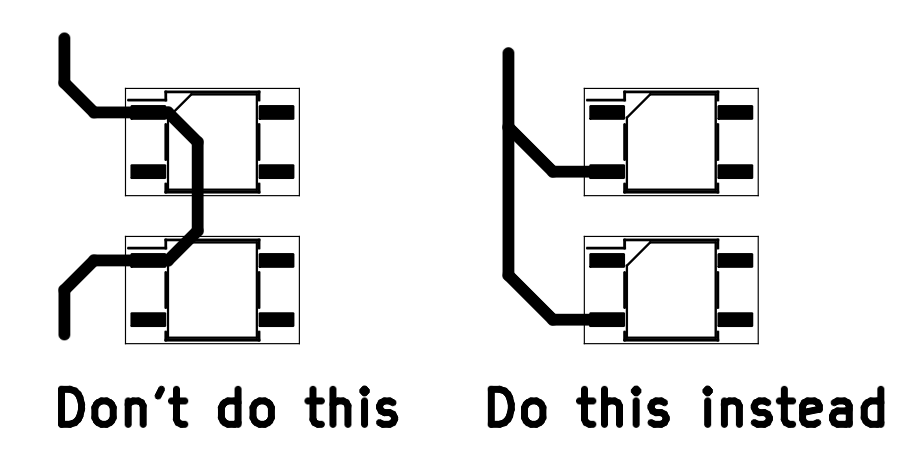
\includegraphics[height=3cm]{power_traces.png}
    \caption{Power trace routing}
    \label{powertraces}
\end{figure}

\item Don't print PCBs at the 3D Printing Center in E5. These are typically poor quality.
\item Make sure that soldermask clearance is set such that there is soldermask between component pads (pay attention to fine pitched components) and that there is no mask on the pads themselves.
\item Thoroughly check the Gerber files for the board before you send them out for fabrication.

\item Points that only apply to designs intended to be hand-soldered:
\begin{itemize}
\item Use SMD pads that are longer than you need. KiCad has specific footprints whose names end in \_HandSoldering, which have extended pads for easier hand-soldering (eg. use "R\_0805\_HandSoldering" instead of "R\_0805".
\item BGA components can't be hand-soldered. We have access to the reflow oven in the 3D print center, but laying paste and inspection will be difficult. Avoid BGA packages if you plan to assemble by hand.
\item Don't batch assemble boards (if you are making multiple) when they arrive, because you will be less inclined to change your design if you notice small bugs if you've already committed lots of components (which are worth far more than the cheap boards) to this design. Build one, test to death, then decide whether to make another revision or to assemble the rest.
\end{itemize}
\end{itemize}
%-- }}}

%Miscellaneous -- {{{
\subsection{Miscellaneous}
\begin{itemize}
\item All switches and connectors need idiot-proof labeling. Labeling should be permanent (i.e. not on tape, etc).
\item All mission critical components should have a hotswappable replacement. You should have that replacement's location written down. "Hotswappable" means you can replace it without any powered tools.
\item If it's conceivably possible for a component to be installed backwards, there should be idiot proof documentation of which way it goes, that documentation should be less than 2 inches from the install point.
\item Buy spares for all components provided it is not prohibitively expensive.
\item All battery connectors should be terminated in a female connector to prevent battery shorting and enable easy battery swapping.
\item Before ordering any components, make a list of all components in your design, and go through their data sheets one by one and ensure that they meet or exceed the requirements of your design. Do not just trust the Digi-Key table values, they are occasionally mislabeled. Design reviewers should also do this.
\end{itemize}
%-- }}}
%-- }}}

%Documentation -- {{{
\section{Documentation Standards}
It is your responsibility to ensure that your project is fully documented and available to the team. Development and documentation for all electrical projects should be tracked in git and hosted on GitHub (under the team organization, waterloo-rocketry). If you manage your repository using issues and pull requests, and if decisions regarding these are made in Slack conversations, put a permalink to the conversation in the issue comment (this is to help traceability). In general, how you manage your project repository is up to you.

Project documentation should include the following:

\begin{enumerate}
\item User's Guide/Checklist
\begin{itemize}
\item Step by step operating instructions.
\item Assume that you will not be there when your system is used.
\end{itemize}
\item Datasheets
\begin{itemize}
\item Self-explanatory. Include datasheets for every component you use.
\end{itemize}
\item Schematics \& Board Layout
\begin{itemize}
\item Any circuit you build should be thoroughly documented in a schematic. Schematics should be correct, clear, and well-organized. The primary purpose of a schematic is to communicate the circuit to someone who hasn't seen it before. A messy schematic will make your circuit harder to review.
\item Some guidelines can be found at \url{https://electronics.stackexchange.com/questions/28251/rules-and-guidelines-for-drawing-good-schematics}.
\item The components in your schematics should match what you intend to use in the circuit. If you are using a particular component, label it as such (and provide a datasheet - see above). This will help identify potential issues in design reviews.
\item Provide both the PDFs and original files for final schematics and PCBs.
\end{itemize}
\end{enumerate}
%-- }}}

%Design Reviews -- {{{
\section{Design Reviews}
If you're designing any part of a system, you should be conducting design reviews. This applies whether there are multiple people working on the system or if you're the only one. If you're alone on a project, this is a good opportunity to make someone else familiar with your work. Apart from resulting in a better circuit, design reviews will also help ensure that you are never the only one who knows how your project should work.
\begin{itemize}
\item  Conduct design reviews on every major revision of your system. This means bringing in another person to discuss your circuit. Keep a record of what was discussed and decided in the review. When presenting a new revision, indicate what has been changed since the last review (a commit message is enough).
\item Design reviews should be thorough. Every component and subcircuit should be checked.
\item Design reviews should be tied to a particular commit in git.
\end{itemize}
%end of design guidelines section -- }}}
\end{document}
